\documentclass{article}

\usepackage{hyperref}
\usepackage{graphicx}
\usepackage{listings}
\renewcommand{\bibname}{参考文献}


\title{\textbf{画图建议指南}}
\author{钟家鑫}
\date{\today}

\begin{document}
\maketitle

\section{简介}
本文档总结了一些科研中画图的建议。
本文的图示提供了相应的代码,请\href{https://github.com/JiaxinZhong/JiaxinZhong.github.io/raw/master/tutorial/plot/plot.zip}{点击这里}下载(在 MATLAB R2023b 中运行通过)。
画图不要求一定使用 MATLAB 完成,很多其他优秀平台也可以使用,但以下提到的要点和思路是相通的。

\section{曲线图}
\label{sec:curves}

曲线图示例见图~\ref{fig:curves}~所示,由附件的 \lstinline!Demo_Curves.m! 文件生成。
主要注意事项包括:
\begin{itemize}
    \item 字体尽可能大,方便读者看清内容。要考虑到论文出版时,图里的字至少不小于正文的字体,还可以适当增大1、2号。
    \item 字体全部用 Times New Roman,统一风格。
    \item 建议 xlabel 和 ylabel 等采用 LaTeX 为 Interpreter。
    \item 输出的图为矢量图,如 *.pdf。
    \item 选择更现代化的颜色方案,如图~\ref{fig:curves}~中使用了 Colorbrewer 中的 Set1 \cite{Brewer2024ColorBrewerColorAdvice}。
    \item 曲线尽量粗一点,如图~\ref{fig:curves}~中的 line width 为 2。
    \item axes 的边框也可以粗一点,如可设为 \lstinline!set(gca, 'linewidth', 1.5)!。
    \item Legend 内容不要挡住曲线。
\end{itemize}

\begin{figure}[!htb]
    \centering
    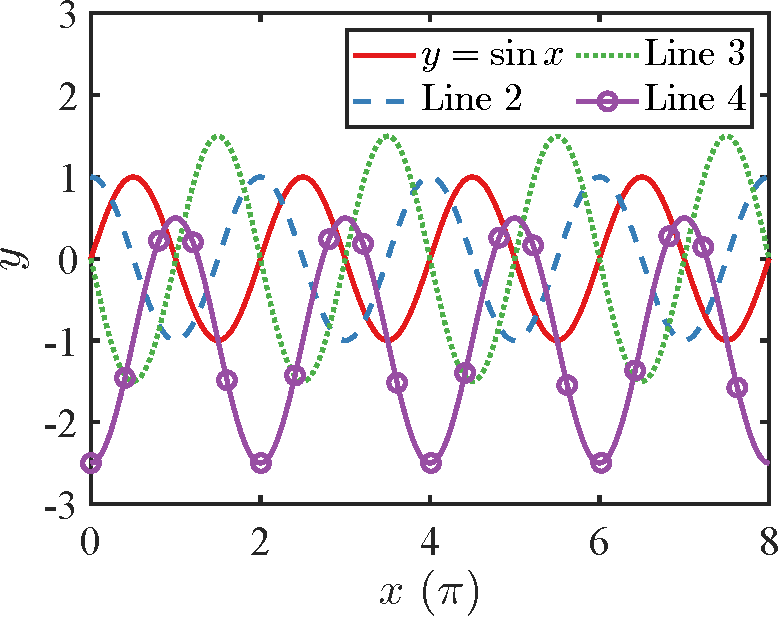
\includegraphics[width = 0.6\textwidth]{Demo_Curves}
    \caption{曲线图示例}
    \label{fig:curves}
\end{figure}


\section{二维图}
二维图示例如图~\ref{fig:2d_fig}~所示,由附件的 \lstinline!Demo_2D.m! 文件生成。
除了第~\ref{sec:curves}~节中的注意事项外,还包括:
\begin{itemize}
    \item 若横纵坐标表示实际物理的长度,则比例应与物理的长度比例相同。如图~\ref{fig:2d_fig}~中长宽比例就当为$8\,\mathrm{m} : 4\, \mathrm{m} = 2:1$。
    \item 选择更现代化的 colormap,图~\ref{fig:2d_fig}~选择的是vik \cite{Crameri2020MisuseColourScience}。
\end{itemize}

\begin{figure}[!htb]
    \centering
    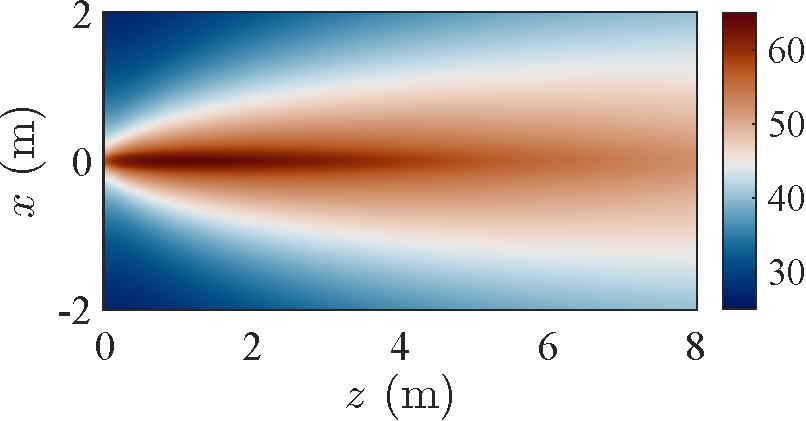
\includegraphics[width = 0.8\textwidth]{Demo_2D}
    \caption{二维音频声场声压级分布图}
    \label{fig:2d_fig}
\end{figure}



% \addcontentsline{toc}{section}{参考文献}
% https://tex.stackexchange.com/questions/261443/changing-bibliography-title-with-biblatex-within-the-document
% \printbibliography[title=参考文献]
\bibliographystyle{unsrt}
\bibliography{bibtex}

\end{document}


